In this chapter, we discuss our working pipeline and system architecture in details.  Generally, our system takes a speech note, textual description or numerical attributes as an input. It processes the input description and outputs the initial human face portrait that corresponds to the given description. Afterwards, the user is allowed to manually control some facial attributes and morphological features and to rotate the face and render it in multiple poses. In the first section, we give an overview about the final system. Then, we discuss the final system architecture in the second section. In the subsequent sections, each module implementation is discussed in details. In the last section, we discuss the other conducted experiments, why we choose this final system and suggestions that can possibly improve the other experiments.

\subsection{Overview and Assumptions}

As mentioned above, our system basically enables the user to describe a human face in words or using numerical values and turns it into a full human face portrait that can be manipulated and rendered in multiple poses. The system relies heavily on generative models and text processing, both are iteratively designed to obtain the required results. The overall flow can be described as follows :
\begin{itemize}
    \item The input speech notes are translated to text.
    \item The textual description (extracted from speech input or manually entered) is processed to extract the numerical values of the required facial features.
    \item The numerical values are used to generate a face embedding vector that encodes the facial attributes in low dimensional space ($512D$).
    \item A generative model is specifically designed to translate from the low dimensional embedding into the full face portrait ($1024X1024$).
    \item The generated face portrait can be further refined by navigating the face embedding space and re-generating the face portrait.
    \item Once the user settles on the final face portrait, the system can render that face in multiple poses to provide further identification.
\end{itemize}

The previous flow provides a very versatile framework to generate face portrait and adjust it to your liking. However, there is an extremely large number of facial attributes and morphological features to describe a human face. Consequently, we have to choose a descriptive subset of these attributes to consider in the face description. We consider $32$ facial attributes for face description, which are listed as follows :
\begin{itemize}
    \item Overall face :
    \begin{itemize}
        \item Gender : Male / Female.
        \item Age : Young / Old.
        \item Thickness : Chubby / Slim.
        \item Shape : Oval / Circular.
        \item Skin Color : Black / White.
        \item Cheeks : Normal / Rosy.
    \end{itemize}
    \item Eyes :
    \begin{itemize}
        \item Color : Black / Blue / Green / Brown.
        \item Width : Wide / Narrow.
        \item Eyebrows : Light / Bushy.
        \item Bags Under Eyes : On / Off.
    \end{itemize}
    \item Nose :
    \begin{itemize}
        \item Size : Big / Small.
        \item Pointy : On / Off.
    \end{itemize}
    \item Ears :
    \begin{itemize}
        \item Size : Big / Small.
    \end{itemize}
    \item Jaw :
    \begin{itemize}
        \item Mouth Size : Big / Small.
        \item Lips Size : Big / Small.
        \item Cheekbones : Low / High.
        \item Double Chin : On / Off.
    \end{itemize}
    \item Hair :
    \begin{itemize}
        \item Color : Black / Blonde / Brown / Red / Gray.
        \item Length : Tall / Short.
        \item Style : Straight / Curly / Receding Hairline / Bald / with Bangs.
    \end{itemize}
    \item Facial Hair :
    \begin{itemize}
        \item Beard / None.
    \end{itemize}
    \item Race :
    \begin{itemize}
        \item White / Black / Asian.
    \end{itemize}
    \item Accessories :
    \begin{itemize}
        \item Glasses : Sight / Sun.
        \item Makeup : On / Off.
        \item Lipstick : On / Off.
    \end{itemize}
\end{itemize}

\newpage

\subsection{System Architecture}

Now, let's discuss our system architecture. The system consists of $6$ modules, $3$ core modules of the project and $3$ auxiliary modules. These modules are deployed in a \emph{web application} to provide an easy-to-use interface for face generation and manipulation. Figure \ref{fig:system} shows the complete block diagram of the system architecture. Meanwhile, figure \ref{fig:app} shows the application design and how the modules are deployed in a web application. The \emph{core} modules are listed as follows :
\begin{itemize}
    \item \textbf{Text Processing :} processes the input textual description and extracts the corresponding numerical values of facial attributes. This problem is similar to \emph{multi-label text classification}, however the outputs are normalized scores of facial attributes, which are designed carefully to match the \emph{face code generation} process.
    \item \textbf{Face Generation :}
    \begin{itemize}
        \item \textbf{Code Generation :} converts the numerical attributes values to be low dimensional face embedding. This is the most \emph{important} and \emph{innovative} module of our system, because it glues the desired attributes scored with the latent space of the generative model (used to generate the face), resulting in more accurate quality outputs.
        \item \textbf{Code-to-Face Translation :} translates the low dimensional face embedding into the actual face portrait. For this purpose, we use \texttt{StyleGAN2}, which is a \emph{state-of-art latent-based generative model}, whose latent space can be manipulated easily to fit our needs.
    \end{itemize}
\end{itemize}

Meanwhile, the \emph{auxiliary} modules are listed as follows :
\begin{itemize}
    \item \textbf{Speech Recognition :} translates the input speech to textual description.
    \item \textbf{Face Refinement :} uses the same generative model to manually refine the generated face portrait through navigating the latent space.
    \item \textbf{Multiple Head Poses Generation :} rotates the generated face portrait and renders it into multiple poses.
\end{itemize}

\begin{figure}[H]
    \centering
    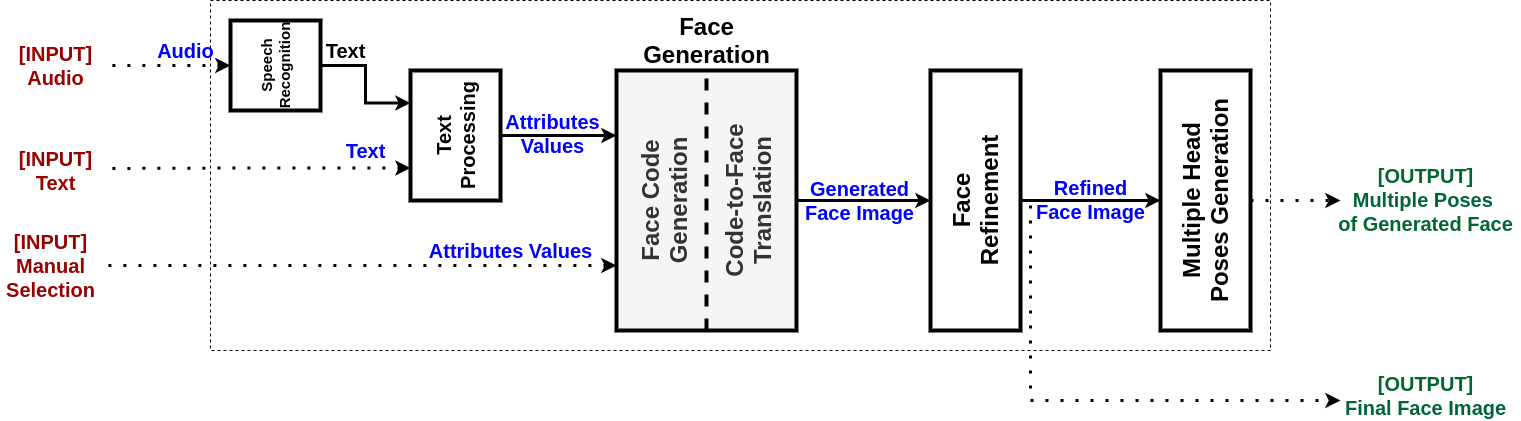
\includegraphics[width=\textwidth]{images/system-design.png}
    \caption{Block diagram of complete system architecture}
    \label{fig:system}
\end{figure}

\newpage

We discuss each module in more details in the subsequent sections. Also, these modules are organized into a web application for easier usage, as shown in Figure \ref{fig:app}. The application is divided into :
\begin{itemize}
    \item\textbf{ Web (Frontend) :} which contains the user interface and, also, the \emph{speech recognizer}. The speech recognizer is moved to the frontend to reduce the network communication overhead between the web application and the server, as transmitting text is easier than transmitting speech. Moreover, the speech recognizer doesn't require high computational power, so it can be embedded in the web application.
    \item \textbf{Server (Backend) :} which is separated into two servers. First server contains the \emph{text processor} and the \emph{generative model} and serves the requests of face generation and refinement. Second server contains the \emph{pose generator} and serves the requests of face rotation.
\end{itemize}

The two servers can communicate with each other to exchange the generated face portraits through \texttt{TCP sockets}. Meanwhile, the web application communicates and sends requests to the servers through \texttt{HTTP REST API}.

\begin{figure}[H]
    \centering
    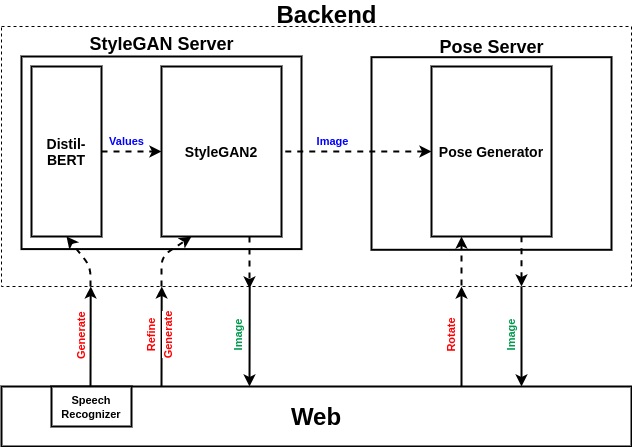
\includegraphics[width=0.8\textwidth]{images/app-design.png}
    \caption{Block diagram of application design}
    \label{fig:app}
\end{figure}

\newpage

\subsection{Module 1 : Speech Recognition}
\label{sec:speech}
This is the first module in our pipeline, its responsibility is to get the textual description of the image from speech. It takes the speech as input then processes it to get its textual content to be used to extract the facial features used to generate the image.

\subsubsection{Functional Description}

Our aim is to add functionality that the user can enter a speech description of the image to generate it, so we used an automatic speech recognition model based on \texttt{DeepSpeech2} \cite{amodei2015deep}, we used the Spectograms features from the audio and applied some preprocessing to those features before training. The target of the speech model is to detect the English spoken words and get their textual meaning so that it can be used to generate the Face Image and output the desired described Face.

\begin{itemize}
    \item \textbf{Input :}
    \begin{itemize}
        \item Speech audio wave.
    \end{itemize}
    \item \textbf{Output :}
    \begin{itemize}
        \item The spoken words on the input audio (textual description).
    \end{itemize}
\end{itemize}

\subsubsection{Modular Decomposition}

\begin{figure}[H]
    \centering
    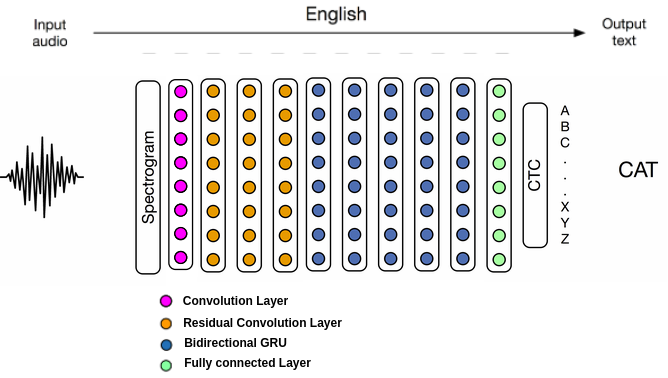
\includegraphics[width=0.8\textwidth]{images/speech.png}
    \caption{Modified DeepSpeech2 network architecture.}
    \label{fig:speechModel}
\end{figure}

As mentioned, we use \texttt{DeepSpeech2} with connectionist temporal classification (CTC) losses as a base to our speech recognition model. The model takes as input features from the audio in the form of spectrograms compressed by frequency and time masking to separate the spectrograms in time and frequency domains. \\
The model architecture (shown in figure \ref{fig:speechModel}) consists of one convolutional layer followed by 3 residual CNNs and 5 bidirectional gated recurrent units GRUs. \\

The first convolution layer used to compress the audio information in low dimension space, The residual CNN consists of layer normalization over the time axis of the speech then 2 convolution layers summed with the original input to the resCNN. \\

The bidirectional RNN uses 512 hidden units used to predict the input character at each time step, The last layer is a fully connected layer to out the final predicted character for each input spectrogram. \\

Connectionist Temporal Classification (CTC) loss function is used to align each character and its location in the audio input file, By summing the probabilities of possible alignments of the input to target and producing a loss value which is differentiable with respect to the model inputs and functions weights. After that those weights are updated using Adam optimizer to minimize this loss value until convergence. \\
\begin{equation}
    L(x,y;\theta) = - \log \sum_{l 	\in Align(x,y)}^{} \prod_{t}^{T} pctc (l_{t} |x;\theta )
\end{equation}

The best aligned character is selected using greedy beam search from all available character to the corresponding input. \\ 
The model Was trained and tested on LibriSpeech ASR corpus which consists of 100 hours for training and test set, "clean" speech for testing. We calculate the word error rate (WER) and character error rate (CER) for the test data to evaluate the model performance.


\subsubsection{Design Constraints}

As our application is a real time interactive app, It’s a must for the speech recognition model to be very fast to be able to process the input quickly so that we gain the users satisfaction. It was a constraint as we couldn't  use larger model with more accurate results, as it will increase the processing time which is against our needs.



\newpage

\subsection{Module 2 : Text Processing}
\label{sec:text}
This module is the first stage in our pipeline that adds the feature of face generation from bare textual descriptions, not just manual manipulators. It's responsible for understanding the input textual description and converting it into facial features logits, where each logit describes how much the generated face should be saturated with. This task is done for 34 different facial attributes where each of them may or may not be entangled with other attributes, such as gender and beard attributes. Attributes may be on different levels as well, some of them are continuous, such as age, some are discrete, such as wearing sunglasses. see figure \ref{fig:scores_example} as an example. 

\begin{figure}[H]
        \centering
        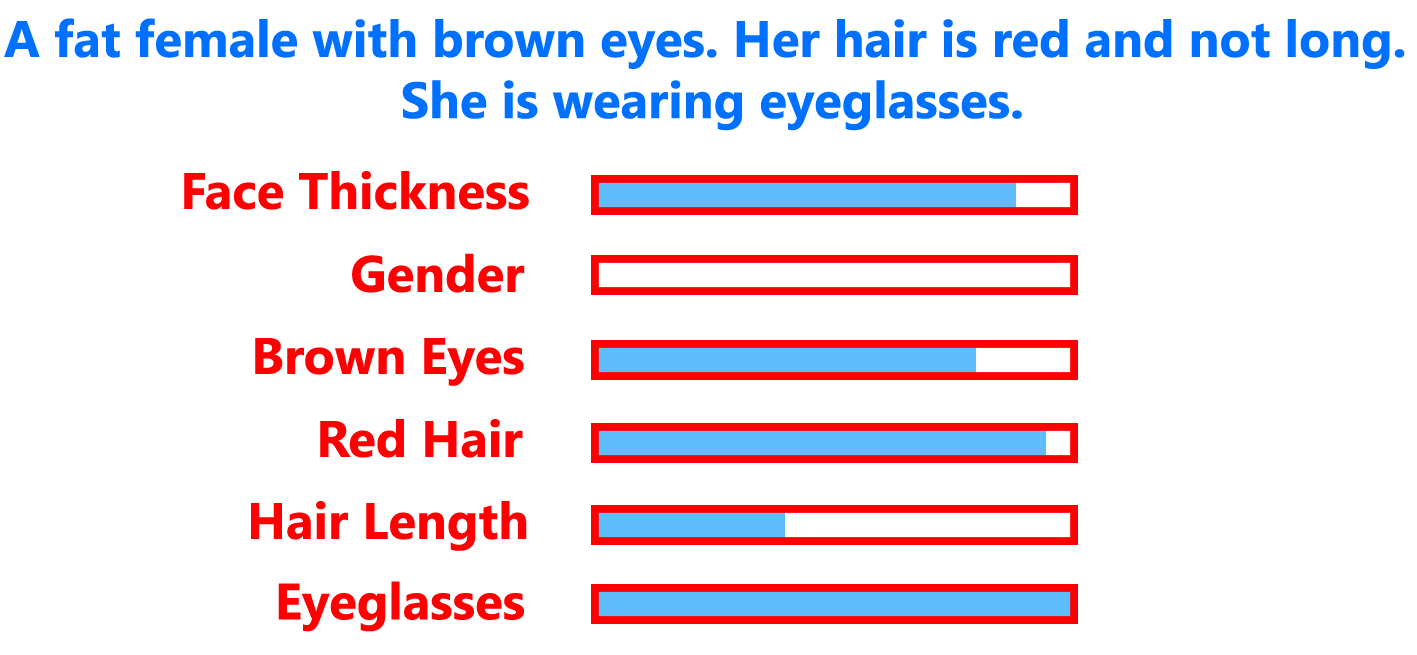
\includegraphics[width=0.8\textwidth]{images/scores-example.png}
        \caption{Attributes Scores Example}
        \label{fig:scores_example}
    \end{figure}


\subsubsection{Functional Description}
This module takes the input text and tries to 
\begin{enumerate}
    \item extract mentioned facial attributes.
    \item extract a score for each mentioned facial attribute referring to the level of saturation of this facial attribute.
    \item extract other non-mentioned attributes.
\end{enumerate}

Here’s the supported list of facial attributes that can be extracted:

\begin{itemize}

    \item Eyebrows
    \begin{itemize}
         \item Bushy Eyebrows               \hspace*{\fill Binary}
    \end{itemize}



    \item Hair Color
    \begin{itemize}
    	 \item Black Hair                   \hspace*{\fill Binary}
    	 \item Red Hair                     \hspace*{\fill Binary}
    	 \item Blonde Hair                  \hspace*{\fill Binary}
    	 \item Brown Hair                   \hspace*{\fill Binary}
    	 \item Gray Hair                    \hspace*{\fill Binary}
    \end{itemize}


    \item Hair Style
    \begin{itemize}
    	 \item Curly-Straight Hair          \hspace*{\fill Continuous}
    	 \item Receding Hairline            \hspace*{\fill Binary}
    	 \item Baldness                     \hspace*{\fill Binary}
    	 \item Bangs                        \hspace*{\fill Binary}
    	 \item Hair Length                  \hspace*{\fill Continuous}
    \end{itemize}


    \item Facial Hair
    \begin{itemize}
    	 \item Beard                        \hspace*{\fill Continuous}
    \end{itemize}


    \item Race
    \begin{itemize}
    	 \item Asian Race                   \hspace*{\fill Binary}
    	 \item Skin Color                   \hspace*{\fill Continuous}
    \end{itemize}


    \item General Facial Attributes
    \begin{itemize}
    	 \item Face Thickness               \hspace*{\fill Continuous}
    	 \item Gender                       \hspace*{\fill Binary}
    	 \item Age                          \hspace*{\fill Continuous}
    	 \item Lips Size                    \hspace*{\fill Continuous}
    	 \item Nose Size                    \hspace*{\fill Continuous}
    	 \item Ears Size                    \hspace*{\fill Continuous}
    	 \item Double Chin                  \hspace*{\fill Binary}
    	 \item High Cheekbones              \hspace*{\fill Binary}   
    	 \item Pointy Nose                  \hspace*{\fill Binary}
    	 \item Rosy Cheeks                  \hspace*{\fill Binary}
    \end{itemize}


    \item Eyes
    \begin{itemize}
    	 \item Black Eyes                   \hspace*{\fill Binary}
    	 \item Green Eyes                   \hspace*{\fill Binary}
    	 \item Blue Eyes                    \hspace*{\fill Binary}
    	 \item Brown Eyes                   \hspace*{\fill Binary}
    	 \item Eye Size                     \hspace*{\fill Continuous}
    	 \item Eye Bags                     \hspace*{\fill Binary}
    \end{itemize}


    \item Makeup
    \begin{itemize}
    	 \item Makeup Saturation            \hspace*{\fill Continuous}
    	 \item Lipstick                     \hspace*{\fill Binary}
    \end{itemize}


    \item Eyeglasses
    \begin{itemize}
    	 \item Sight Glasses                \hspace*{\fill Binary}
    	 \item Sun Glasses                  \hspace*{\fill Binary}
    \end{itemize}

\end{itemize}



\subsubsection{Modular Decomposition}
This module is considered as an NLP task that can be tackled using classical approaches, such as Text Parsing and Tagging, and Deep Learning approaches. The final design for this module is to use the power of Deep Learning approaches especially transformers to analyze and understand the text. This is because that the classical approaches failed in such a task as there are a lot of sequence dependencies on the textual description that may arise such as restricting the age of the described person to the range of low-to-medium beard levels and gender attribute, except in the case of age attribute is mentioned explicitly or implicitly in the text, for example "a boy", "a boy with a beard" and "a boy almost in his thirties", the first description should be understood as a child or teenager, while other descriptions refer to a middle-aged man. a lot of other dependencies that may arise that make the classical approaches not feasible and makes the deep learning solutions a must to tackle such a task. 
\\
\\
The biggest challenge in the Deep Learning approaches is that there are no available datasets mapping textual descriptions to facial features. That’s what led us to use synthesize our own dataset that must be much likely to be human-generated. This what made the module to be split into two sub-modules as shown in figure \ref{fig:text_processing_pipeline}. First one is the Dataset Synthesis sub-module and the Deep Learning Sequence Model to be trained on the synthesized dataset.


\begin{figure}[H]
        \centering
        
\includegraphics[width=0.8\textwidth]{images/text-processing-submodule.png}
        \caption{Text Processing Pipeline}
        \label{fig:text_processing_pipeline}
    \end{figure}

\paragraph{Dataset Synthesis sub-module}
This sub-module is the most critical one, as it should be as likely as possible to be human-generated. The approach we used to do so consists of three main stages as shown in figure \ref{fig:dataset_syn} in the reverse order of what needed in the training phase.

\begin{figure}[H]
        \centering
        
\includegraphics[width=0.8\textwidth]{images/data-synthesis.png}
        \caption{Dataset Synthesis Pipeline}
        \label{fig:dataset_syn}
    \end{figure}

\begin{enumerate}
    \item Random Attribute Generation
    
        In this stage, we generate any random attribute scores for all 34 attributes. Each attribute is generated with its pre-defined range of scores with one of random different modes
        
        \begin{itemize}
            \item Full Random Mode: All attributes will be mentioned in the text with random scores.
            
            \item Half-Length Random Mode: 50\% of attributes will be mentioned in the text with random scores, while other 50\% will not be mentioned.
            
            \item Short Random Mode: 20\% of attributes will be mentioned in the text with random scores, while other 80\% will not be mentioned.
            
            \item Very-Short Random Mode: 10\% of attributes will be mentioned in the text with random scores, while other 90\% will not be mentioned.
        \end{itemize}
        
        Mentioned Attributes are generated with some restrictions to make their scores consistent with others, such as
        \begin{itemize}
            \item Females, babies and children cannot have facial hair.
            \item Females cannot be bald.
            \item Males and babies cannot put makeup or lipstick.
            \item Bald people cannot have any hair attribute mentioned, such as hair color or hair style.
            \item One hair color at most can be mentioned (i.e. no person can have both yellow and red hair).
            \item One eye color at most can be mentioned (i.e. no person can have both blue and black eyes).
            \item People with bangs cannot have receding hairline and vice versa.
            \item One Eyeglasses type at most can be mentioned (i.e. no person wear both sun and sight glasses).
        \end{itemize}
    
    
    \item Random Textual Die Generation
    
    In this sub-module, a textual description is generated in a textual die using the random scores of facial attributes. Attributes are categorized using different categories, such as
    
    \begin{itemize}
    \item First Categorization is based on the facial part that is described, such as all hair attributes (Black Hair, Blonde Hair, Gray Hair, Red Hair, Brown Hair, Straight Hair, Hair Length) can be combined in a single description of the hair (e.g. a woman with long, brown and curly hair).
    \item Second Categorization is based on the grammatical way that the attribute can be described with. Each attribute can be of one or more of types below
        \begin{itemize}
            \item With Attributes: attributes that can be described using with statement (e.g. a man with brown hair and blue eyes.)
            \item Has Attributes: attributes that can be described using has statement (e.g. a man who has brown hair and blue eyes.)
            \item Puts Attributes: attributes that can be described using put statement (e.g. a woman is putting heavy makeup.)
            \item Wears Attributes: attributes that can be described using wear statement (e.g. a woman is wearing a glasses.)
            \item Full Statement Attributes: attributes that can be described using a full statement (e.g. His hair is brown. His Eyes is blue)
            \item Adjective Attributes: attributes that can be described using adjectives (e.g. a blond old man.)
        \end{itemize}    
    \end{itemize}
    
    Each mentioned attribute can have a form of different forms, such as
    \begin{itemize}
        \item Positive Attributes using Synonyms: describing an attribute with one of its synonyms randomly (e.g. “a man with a thick face.” can be described as a “a chubby man.”).
        \item Positive Attributes using Antonyms and Negation: describing an attribute with the negation of one of its antonyms randomly (e.g. “a man with a thick face.” can be described as a “He is not thin” or “a man with non-thin face.” and so forth).
        \item Negative Attributes using Antonyms: describing a negative attribute with one of its antonyms randomly (e.g. “a man with no thick face.” can be described as a “a thin man.”).
        \item Negative Attributes using Synonyms and Negation: describing a negative attribute with the negation of one of its synonyms randomly (e.g. “a man with no thick face.” can be described as a “He is not chubby” or “a man with non-thick face.” and so forth).
    \end{itemize}
    
    Each mentioned attribute chooses one of its categories and one of its forms randomly and reserve a slot in the textual die represented in figure \ref{fig:textual_die} .
    
    
    \begin{figure}[H]
        \centering
        
\includegraphics[width=0.8\textwidth]{images/textual-die.png}
        \caption{Textual Die where each attribute chooses a random slot for itself}
        \label{fig:textual_die}
    \end{figure}
    
    
    \item Paraphrasing
    
    
    As we use deep learning approaches, using the textual die to train a model is just making the model learn the die itself, not to generalize and extract the attributes from any other textual description. So, in this sub-module, we tried different approaches to restructure and paraphrase the textual die generated in the previous step, so that the generated description is more likely to be human-generated and to be general. To do so, we tried two approaches as a paraphraser
    
    \begin{itemize}
        \item First Approach: Training a Sequence-To-Sequence model using the “entailment” class in Stanford Natural Language Inference Dataset (SNLI) to re-structure any English statement to any other English statement based on the diversity of expressing ways in the English Language
        \item Second Approach: Using a random cycle of machine translators (e.g. translates the die in the sequence “English To Arabic To Spanish To Italian To English” or in the sequence “English To Chinese To English”). Using the power of different linguistic ways in different languages makes the paraphrased description more generic. 
    \end{itemize}
\end{enumerate}

\paragraph{Deep Learning Sequence Model}

The main task of Text Processing module is to map input textual description to corresponding attributes scores, so It’s a multi-class multi-label NLP problem. Therefore, in this sub-module we trained different deep learning architectures on the previously generated dataset. We tried 

\begin{itemize}
    \item LSTM Architecture: 2 BiLSTMs followed by a linear layer.
    \item Transformers Architecture: DistelBert-base-uncased, Bert-base-uncased, Albert-base-v2, Roberta-base
\end{itemize}

Where transformers architectures out-performed, so the final choice was DistelBert-base-uncased, as it’s the lightest one out of them with accuracy hit +99\% on validation.



\subsubsection{Design Constraints}
The design constraints of this module are enumerated as follows :
\begin{itemize}
    \item Human-like Dataset Synthesis: The biggest challenge of this module is that there’s no available dataset to tackle such a task. So, we needed to synthesize our own dataset that should be as generic and human-generated as possible, so that what made the paraphraser performance really matters.
    \item Conditional entailment of different facial attributes: as different facial attribute may affect each other, so the dataset should be generated in a robust way so that it can train the deep learning model to detect such relations, such as entanglement between beard, gender and age.
    \item Accuracy matters: as this is one of the early modules in the pipeline, the results of all other modules depend on its performance and accuracy. So, lack of accuracy in this module will be catastrophic for the whole pipeline.
\end{itemize}



\newpage

\subsection{Module 3 : Face Code Generation}
\label{sec:code_gen}
Here, we discuss the face code generation from numerical values of facial attributes. This is the most important and innovative module in our system and the first stage of \emph{face generation}. It's worth \textbf{noting} that we use both of the terms \emph{"feature"} and \emph{"attribute"} to refer to a facial attribute, like hair color or nose size.

\begin{figure}[H]
    \centering
    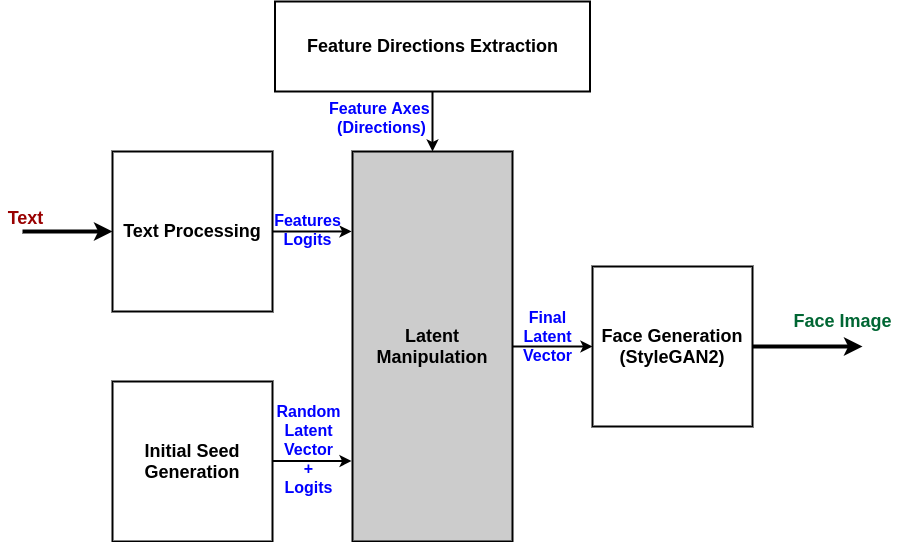
\includegraphics[width=0.8\textwidth]{images/face-gen-arch.png}
    \caption{Detailed block diagram of the three core modules workflow}
    \label{fig:face_gen}
\end{figure}

\subsubsection{Functional Description}

Figure \ref{fig:face_gen} shows a block diagram of the interaction between the $3$ core modules. We can see that the code generation module is the main driver of our face generation process. Generally, it converts the numerical attributes values (a.k.a. \emph{logits}) into a face embedding vector that matches the design of the latent space of the face generator (\emph{StyleGAN2}). Basically, it starts from an initial vector and uses the \emph{required feature values} and \emph{extracted feature directions} to transform this vector into the final latent vector, which is passed to the generative model.

\begin{itemize}
    \item \textbf{Input :}
    \begin{itemize}
        \item Numerical values of facial features (logits).
    \end{itemize}
    \item \textbf{Output :}
    \begin{itemize}
        \item Low dimensional face embedding vector (latent vector).
    \end{itemize}
\end{itemize}

\subsubsection{Modular Decomposition}

As figure \ref{fig:face_gen} tells, the code generation module can be torn down into $3$ sub-modules, which are \textbf{latent manipulation}, \textbf{initial seed generation} and \textbf{feature directions extraction}. Each sub-module is discussed in details to show how they integrate to each other to achieve the desired goal.

\paragraph{Feature Directions Generation}
Since, we use \texttt{StyleGAN2} \cite{karras2020analyzing} as our generative model, we have a full $512D$ latent space that is used to encode the whole face attributes. The changes in this latent space maps to the generated face image and similar features occupies the same area in the latent space. Consequently, we have to come up with a way to extract the axes (\emph{hyperplanes}) in this latent space to define each of our $32$ facial features. These feature directions are, then, used to manipulate the latent vector, in order to map to the required face image. 

\begin{figure}[H]
    \centering
    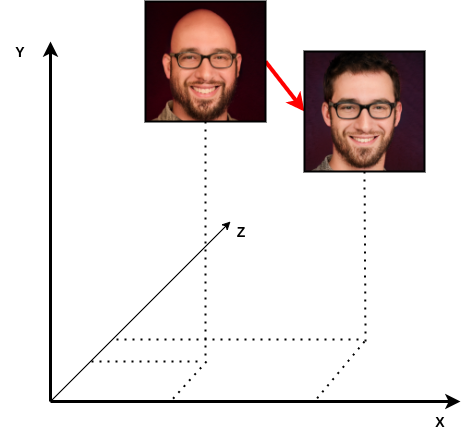
\includegraphics[width=0.5\textwidth]{images/feature-dir.png}
    \caption{Illustration of feature directions in latent space}
    \label{fig:feature_dir}
\end{figure}

Figure \ref{fig:feature_dir} further illustrates the idea of feature directions in the latent space. Here, we plot two face images in a $3D$ latent space. We can see that the difference between the two images in the existence and the absence of the hair, thus the red arrow represents the \emph{baldness} feature direction in that $3D$ latent space (moving along this particular vector causes hair density to change).

Our method of extracting the feature directions (\emph{hyperplanes}) consists of $3$ steps :
\begin{enumerate}
    \item \textbf{Code-Image Pairs Generation and Classification :} First, we use \texttt{StyleGAN2} to generate a large number of synthetic faces from random latent vectors. After so, we cluster the synthetic images (along with their latent vectors) according to each feature. The clustering can be based on discrete categories (like \emph{hair color} or \emph{race}) or continuous values (like \emph{hair length} or \emph{nose size}). We randomize the synthetic images in each clustering process to have better generalization and to cope with potential generation noise. For classification and regression, we use one of three possible methods, which are \textbf{manual labelling}, \textbf{classical image processing techniques} and \textbf{neural networks}. Thus, the output of this process is different groups of synthetic images sharing common facial features, along with their latent vectors.
    
    \item \textbf{Feature Directions Fitting :} Now, we have a set of latent vectors (\texttt{X}) and their corresponding feature values (\texttt{Y}). It's required to find a set of feature directions that satisfies the mapping between feature vectors and values. This problem can be formulated as :
    \begin{equation}
        Y = A_f \cdot X
    \end{equation}
    Where $A_f$ is the axis (direction) of feature $f$. \\
    We can obtain the solution to this equation in a closed form. However, due to the noise in both generation and classification, along with the non-linear nature of the problem, we opt to use \emph{ML} methods, specifically \textbf{Logistic Regression} and \textbf{SVM} to get an \emph{approximate solution}. Meanwhile, we cannot see any difference between the two methods, as they yield almost the same results. \\
    Finally, the generated feature directions are normalized to unit vectors :
    \begin{equation}
        A_{unit} = \frac{A}{||A||}
    \end{equation}
    
    \item \textbf{Directions Orthogonalization :} Facial features entanglement is one of the most difficult challenged of face generation. Some attributes in the human face tend to be extremely entangled by nature. For example, Asians rarely have curly hair, a woman cannot have beard and a man cannot put on makeup. Since \texttt{StyleGAN2} is trained and tuned on \textbf{FFHQ} dataset \cite{karras2019stylebased}, which contains real human faces, it is normal to notice some entanglement between some features. Consequently, the feature directions have to be further disentangled by using \emph{orthogonalization}. The orthogonalization process is done iteratively, starting from the most accurate feature directions. We orthogonalize other feature directions on the accurate ones, so that we have completely independent feature directions, where tuning one direction doesn't affect the others. The directions are orthogonalized as follows :
    \begin{equation}
        A_{proj} = (A \cdot B_{unit}) B_{unit}
    \end{equation}
    \begin{equation}
        A_{orthogonal} = A - A_{proj}
    \end{equation}
    
    Figure \ref{fig:ortho} visually illustrates the \emph{directions orthogonalization} process on $2D$ vectors.
    
    \begin{figure}[H]
        \centering
        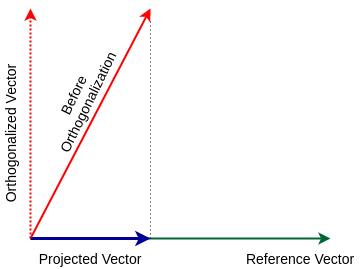
\includegraphics[width=0.5\textwidth]{images/orthogonalization.png}
        \caption{Illustration of orthogonalization relative to a reference vector}
        \label{fig:ortho}
    \end{figure}
    
    To ensure convergence to reasonable set of feature directions, we use a threshold margin to stop the orthogonalization process, which is from $85$ to $95$ degrees ($5$ degrees on each side of normal angle).
\end{enumerate}

\paragraph{Initial Seed Generation}
In order to avoid noise and discontinuities in the latent space, we generate an initial random latent vector. This is done by generating a random $512D$ vector and then passing it through the \emph{mapping network} of \texttt{StyleGAN2}, which is not invertible. This initial vector is, then, manipulated by sequential navigation along each feature direction (axis) with certain amounts. To get these amounts, we should know the component of the initial vector along each feature direction. We do that by simply performing a dot product between the initial vector and the unit vector of each feature direction. Thus, we have an initial latent vector and the numerical attributes values, it presents. 

\paragraph{Latent Manipulation}
This sub-module ingests all the inputs and produces the required latent vector (\emph{face embedding}) that describes all of the required facial attributes. The inputs to this latent manipulation sub-module are \emph{initial random vector} along with its logits, \emph{text logits} and \emph{feature directions}. The latent manipulation, simply, wants to realize the following transformation on the \emph{initial random vector} :
\begin{equation}
    E_{final} = E_{initial} + (l_{text} - l_{rand}) D
\end{equation}
Where $E_{final}$ is the final latent (\emph{embedding}) vector of dimensions $1X512$, $E_{initial}$ is the initial random vector of dimensions $1X512$, $l_{text}$ is the text logits vector of dimensions $1X32$ (remember that we consider $32$ facial features), $l_{rand}$ is the logits vector of the initial random vector of dimensions $1X32$ and $D$ is the feature directions matrix of dimensions $32X512$. The transformation includes calculating the difference between the required logits and the random logits and, then, use this difference to move the initial random vector along the feature directions to reach the final latent vector.

It might seem straight forward to perform this transformation. Unfortunately, it's not feasible to perform the transformation using direct matrix multiplication, mainly due to heavy \emph{entanglement} between direction vectors even after \emph{orthogonalization}. Also, the latent space of \texttt{StyleGAN2} can be very noisy in certain regions, so transformations have to be done carefully. 

Consequently, the processing in this sub-module is done iteratively as follows :
\begin{itemize}
    \item Both random and text logits are scaled from $0$ to $1$, which cannot have significant effect, when navigating using unit directions. Consequently, the inputs logits are scaled with the directions scale, which is obtained empirically to be from $-4$ to $4$, as shown in figure \ref{fig:dir_scale}.
    \item The next step is to get the \emph{difference} between \emph{text logits} and \emph{random logits}, which is of dimensions $1X32$. We call that \textbf{differentiated logits}. It's worth noting here that the input text usually contains a \emph{subset} of the facial features. Consequently, \emph{not all} the text logits are set to specific values. So, when doing the \emph{differentiation}, we set the differentiated logits of the \emph{unmentioned facial features} to $0$. So, it can be summarized as follows :
    \begin{equation}
        l_{diff}=
        \left\{ \begin{array}{ll}
            l_{text} - l_{rand} & l_{text} \neq None \\
            0 & \text{otherwise}
        \end{array} \right.
    \end{equation}
    \item Loop over each direction in feature directions :
    \begin{itemize}
        \item Multiply the \emph{differentiated logit} corresponding to the \emph{current feature} with its \emph{direction}.
        \item Add the product to the current latent vector (starting with the \emph{initial random vector}). The following equation summarizes these steps :
        \begin{equation}
            E_{next} = E_{prev} + l_{diff}[j] * D[j]
        \end{equation}
        \item Finally, to ensure that every transformation is independent of the subsequent transformations and that they are applied sequentially, we re-compute the \emph{produced latent vector logits} and re-differentiate it with the \emph{text logits}. This is done on every iteration of the latent manipulation process.
    \end{itemize}
\end{itemize}

\begin{figure}[H]
    \centering
    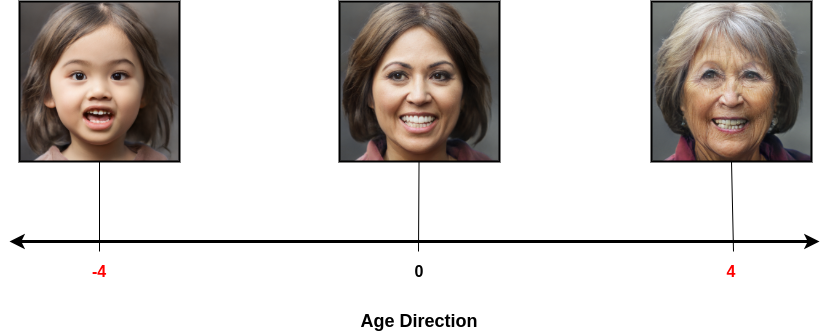
\includegraphics[width=0.8\textwidth]{images/dir-scale.png}
    \caption{Illustration of directions scale using age direction}
    \label{fig:dir_scale}
\end{figure}

By applying the previous process, the \emph{numerical value} of facial features extracted from text or manually entered by the user can be converted into a complete face embedding (\emph{latent vector}) matching the required facial attributes. This vector can be passed to \texttt{StyleGAN2} to translate it to a complete human face image.

\subsubsection{Design Constraints}

The design constraints of this module are enumerated as follows :
\begin{enumerate}
    \item \textbf{Facial attributes entanglement} is the main challenge of the face code generation module. Naturally, human face attributes are related to each other. For example, Asians barely have curly hair, no woman cannot have beard and most women have long hair and wear makeup. We mentioned before that \texttt{StyleGAN2} is trained and refined on \texttt{FFHQ} dataset, which contains real human faces. Consequently, it's normal to see heavy entanglement between features in the latent space. Due to this \emph{entanglement}, we have to perform extra computations to get decent results.
    \item \textbf{Random initialization} of the latent vector can cause some issues with the final output, as the vector can be initialized in a noisy area of the latent vector. We try to \emph{limit} the initialization of latent vector to a certain set of random vectors to avoid this effect. This method significantly reduces the \emph{random initialization effect}, however it's not fully cured.
    \item \textbf{Directions accuracy} can be a challenge as well. Some factors can negatively affect the feature directions accuracy. These factors include \textbf{synthetic image clustering} (whether \emph{classification} or \emph{regression}) and \textbf{directions fitting} process. We already discussed our solutions to this problem.
\end{enumerate}

\subsubsection{Synthetic Image Clustering}

As we mentioned before, it's required to cluster the generated synthetic images, in order to be able to fit the feature directions. The \emph{clustering} process can be performed through \emph{classification} or \emph{regression}. For example, features like hair and skin colors should be classified (grouped) into discrete categories, however features like hair length and mouth size should be assigned a continuous value. We do this task using one of three different methods :
\begin{enumerate}
    \item \textbf{Manual labelling} is the first idea to come to our minds. It's straight forward to manually classify a group of faces according to a certain feature. This method is used with some features, however it's very cumbersome and only works for classification.
    \item \textbf{Classical image processing techniques} are, also, used to classify images based on some features. Mainly, we use these techniques to detect \emph{colors} like eye color and hair color. We use \emph{morphological operators} and \emph{classical segmentation} to detect \emph{the eye} or \emph{the hair} and then retrieve its color.
    \item \textbf{Deep learning techniques} (\emph{neural networks)} are used to perform regression on the rest of the features. We basically use \emph{facial landmark detection} pretrained networks to detect the important facial landmarks, which is, then, used to calculate \emph{sizes} and \emph{distances}.
\end{enumerate}


\newpage

\subsection{Module 4 : Code-to-Face Translation}
\label{sec:face_gen}
 Here, we discuss the process of converting the face embedding (\emph{latent vector}) to a complete face image using \texttt{StyleGAN2} (our chosen generative model). We discuss our reasons for choosing this particular architecture and how we use it.

\begin{figure}[H]
    \centering
    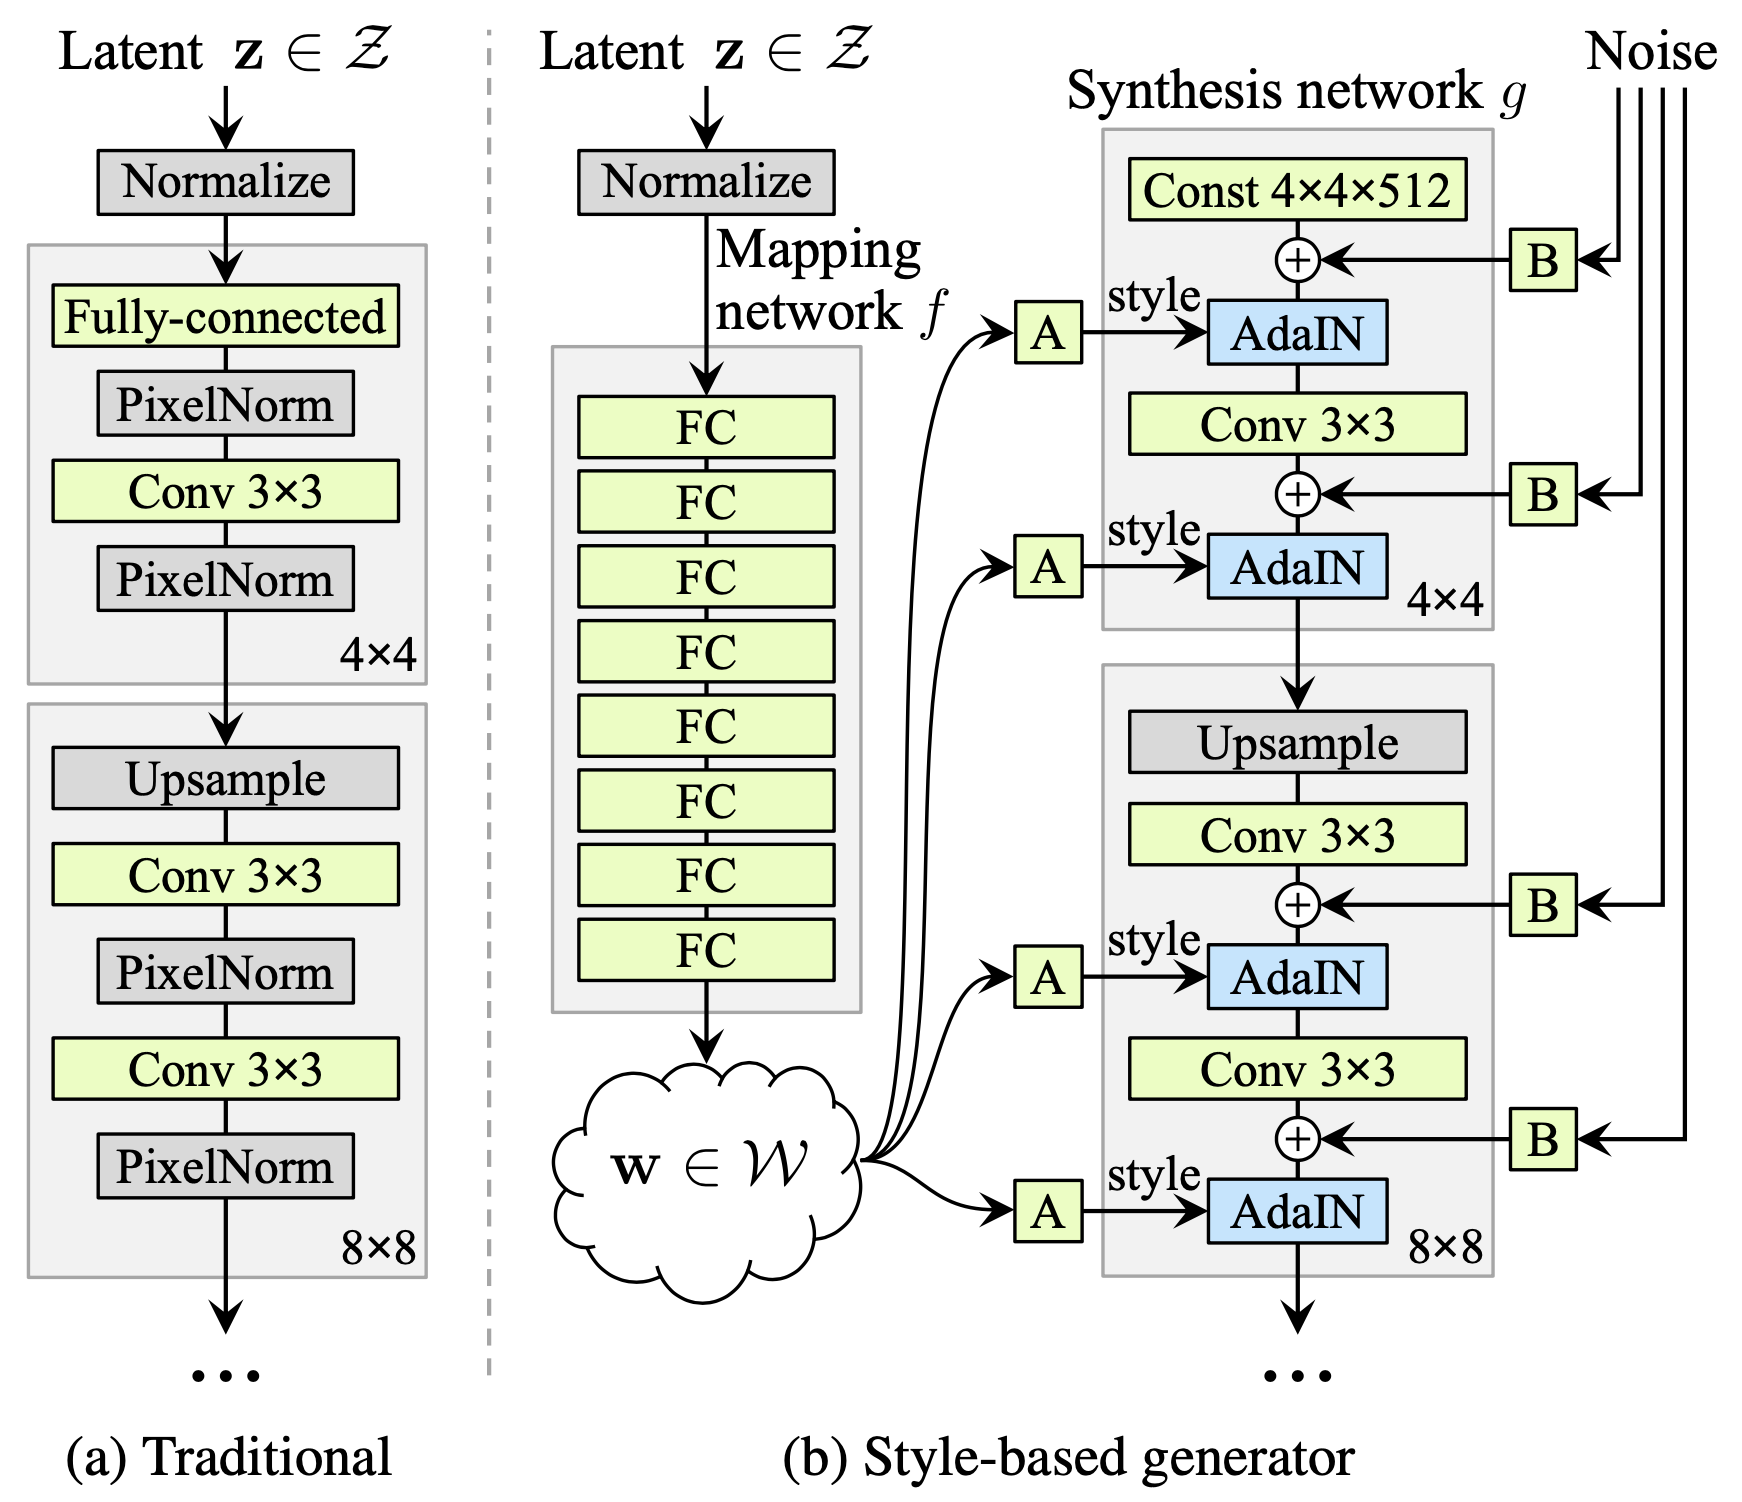
\includegraphics[width=0.7\textwidth]{images/stylegan.png}
    \caption{Style-based GAN architecture against traditional GAN}
    \label{fig:stylegan}
\end{figure}

\subsubsection{Functional Description}

This module utilizes the power of \emph{style-based} generative models, specifically \texttt{StyleGAN2} \cite{karras2020analyzing}, to translate the required \emph{latent vector} to a complete \emph{human face image}. \emph{Style-based GANs} (sometimes called \emph{latent-based GANs}) can exert artistic control over the generated content (images, videos, text ..., etc). Consequently, we can tune it to fit our need and, iteratively, design it along with \emph{code generation} \ref{sec:code_gen} and \emph{text processing} \ref{sec:text}, in order to have a complete end-to-end pipeline for \emph{text-to-face generation}.

\begin{itemize}
    \item \textbf{Input :}
    \begin{itemize}
        \item Low dimensional face embedding vector (latent vector).
    \end{itemize}
    \item \textbf{Output :}
    \begin{itemize}
        \item Complete human face image (portrait).
    \end{itemize}
\end{itemize}

\subsubsection{Modular Decomposition}

As mentioned before, we opt to use \emph{Style-based GANs} to be able to artistically control the output and designed the whole pipeline for \emph{text-to-face generation}. Moreover, we choose \texttt{StyleGAN2}, because it's one of the most popular and robust Style-based GANs in research literature. Also, it's relatively lightweight compared to other GANs used for the same purposes, but most importantly, \texttt{StyleGAN2} excels at human face generation based on latent space. Figure \ref{fig:stylegan} shows the original architecture of \texttt{StyleGAN} and how it is compared to traditional GANs. \texttt{StyleGAN} generator has two networks as follows :

\begin{itemize}
    \item \textbf{Mapping network} creates nonlinear transformation to the input latent vector $z$ ($512D$). This transformation is not invertible and results in a $512D$ latent vector $w$. This latent vector $w$ is expanded into several $512D$ vector using affine transformation, which gives the \emph{extended latent vector} $w+$. The extended latent vector $w+$ dimensions depend on the dimensions of the output image.
    \item \textbf{Synthesis network} generates the synthetic image from \emph{normally-distributed noise} guided by the extended latent vector $w+$.
\end{itemize}

\texttt{StyleGAN2} \cite{karras2020analyzing} is a newer version that follows the same architecture, but with some modifications to further improve the control over latent space and the quality of the outputs. 

So, let's discuss how we adapted \texttt{StyleGAN2} to our work :

\begin{itemize}
    \item To provide a high fidelity results, we target $1024X1024$ synthetic images. To achieve this, we have to use an extended latent vector $w+$ of dimensions $18X512$, meaning we repeat the latent vector $w$ $18$ times with \emph{affine transformation} for each.
    \item To further improve feature directions disentanglement, we fine-tune \texttt{StyleGAN2} using a subset of \texttt{FFHQ} dataset with increasing the weight of \emph{perceptual path regularization} in the loss function. \emph{Perceptual path regularization} in \texttt{StyleGAN2} loss encourages the smooth mapping between latent and image spaces. So, when increasing it in certain directions, it highly penalizes the deviation between latent and image spaces in these directions giving more organized latent space. To avoid using the whole dataset, we use \texttt{StyleGAN2} \emph{adaptive discriminator augmentation} (\textbf{ADA}) \cite{karras2020training} training methodology.
    \item Finally, we opt to remove the \emph{mapping network} of \emph{StyleGAN2} generator and only use the \emph{synthesis network}. This is mainly because :
    \begin{itemize}
        \item The mapping network doesn't satisfy the \emph{path length regularization}, so there is no smooth mapping between latent space $z$ and image space (only with latent space $w$). This is discussed in the original paper \cite{karras2020analyzing} and our experiments support that.
        \item The mapping network is not invertible, unlike the synthesis network. So, we cannot reverse the transformation from image space to latent space $z$. That's why we only work with latent space $w$ to test the consistency of the results.
        \item Removing the mapping network reduces the computations and the memory footprint, which is crucial in our case.
    \end{itemize}
\end{itemize}

After the previous modifications, the output model can directly translate the face embedding vector (\emph{latent space}) into a complete human face portrait. 

Notice that using this methodology of \textbf{code-to-face translation} along with \textbf{code generation} makes the sequential navigation in the latent space is \emph{easily invertible}, which eases the generation and the refinement (discussed in \ref{sec:face_ref}) of the synthetic face and gives the system versatility and fault tolerance. Figure \ref{fig:latent_nav} illustrates the idea of \emph{invertibility} of sequential edits on a $2D$ latent space example. Here, we show a simplified $2D$ latent space with $3$ feature direction. $AB$ vector represents the \emph{hair color} direction and $BC$ vector represents the \emph{gender} direction. Point $A$ starts with a \emph{blonde girl}, moving along $AB$ vector results in a \emph{girl with black hair} at point $B$. Then, moving along $BC$ vector gives us a \emph{man with black hair} at point $c$. Consequently, moving along $CA$ vector, which is the opposite of the resultant of $AB$ and $BC$, gives us the original face, thus inverting the sequential changes.

\begin{figure}[H]
    \centering
    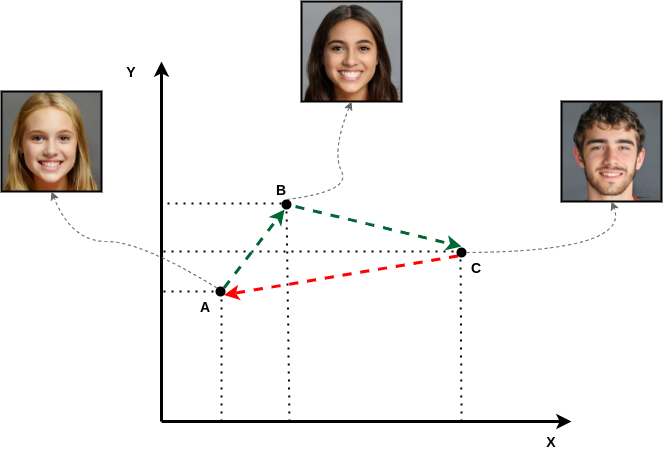
\includegraphics[width=0.7\textwidth]{images/latent-nav.png}
    \caption{Illustration of sequential navigation and invertibility in a $2D$ latent space}
    \label{fig:latent_nav}
\end{figure}

\subsubsection{Design Constraints}

The basic design constraints for this module can be enumerated as follows :

\begin{enumerate}
    \item \textbf{Network size} is surely one of our challenges. \texttt{StyleGAN2} has a large memory footprint, as the case with most \emph{deep generative models}. This constrains its training and deployment. We managed to remove the \emph{mapping network}, which gives us a change to use the full \emph{synthesis network}.
    \item \textbf{Faces dataset} is, also, a constraint, because real images of human faces contains entanglement between facial features (\emph{as discussed before}). So, we have to exert extra effort in the \textbf{code generation} module to solve some of this entanglement, emerging from real human faces datasets.
\end{enumerate}


\newpage

\subsection{Module 5 : Face Refinement}
\label{sec:face_ref}
\subsubsection{Functional Description}

\subsubsection{Modular Decomposition}

\subsubsection{Design Constraints}

\subsubsection{Other Description}

\newpage

\subsection{Module 6 : Multiple Head Poses Generation}
\label{sec:poses}
\subsubsection{Functional Description}

\subsubsection{Modular Decomposition}

\subsubsection{Design Constraints}

\subsubsection{Other Description}

\newpage

\subsection{Module 7 : Web Application}
\label{sec:web_app}
\subsubsection{Functional Description}

\subsubsection{Modular Decomposition}

\subsubsection{Design Constraints}


\newpage

\subsection{Other Approaches}
\label{sec:other_app}
At the beginning of our project, we tried to automate the whole pipeline in an \emph{end-to-end} deep learning approach starting from the textual input to the generated face. The pipeline is shown in figure \ref{fig:old}.

\begin{figure}[H]
    \centering
    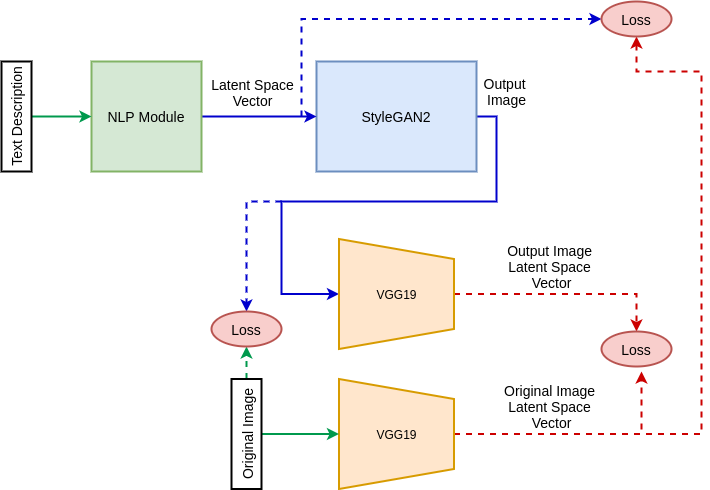
\includegraphics[width=0.7\textwidth]{images/old.png}
    \caption{Old Approach}
    \label{fig:old}
\end{figure}

\subsubsection{Face Generator Module}

We used the same latent-based generative model, which is \texttt{StyleGAN2} with no modifications. We aimed to use the generator pretrained weights to start the \emph{end-to-end} training process, which tunes the generator weights along with the whole system.

\subsubsection{NLP Module}

This module translates the text directly to the \texttt{StyleGAN2} latent vector $z$ that encodes all described facial features. We used a simple \emph{Recurrent Neural Network} (RNN) architecture that consists of $2$ recurrent layers followed by a fully connected layer. This is trained on a semi-synthesized dataset of text, latent vector and face image triplets.

\subsubsection{Dataset and Training}

Our dataset generation and the training process goes as follows :

\begin{itemize}
\item We started by using \emph{Face2Text} dataset that consists of $4000$ records of textual descriptions of images in the \emph{CelebA} dataset.
\item This dataset is very small, so we needed to make it larger :
\begin{itemize}
    \item We used \texttt{FaceNet} \cite{Schroff_2015} to encode the whole \emph{CelebA} dataset, as \texttt{FaceNet} is one of the best facial features extractors.
    \item We used \emph{K-Nearest Neighbors} (KNN) to get the closest $10$ matches of each celebrity in \emph{Face2Text} dataset from \emph{CelebA} dataset.
    \item Then, we manually picked the best $5$ matching faces out of the $10$ faces got from KNN. Therefore, we have a dataset of $20,000$ text-face pairs.
    \item We separately trained a strong feature extractor (\texttt{VGG19}) to map from face images to latent vector, which we called \emph{image-to-latent projector}.
    \item Finally, we used the image-to-latent projector to generate the latent vector corresponding to the dataset faces.
    \item Thus, we had the final dataset triplets of text, latent vector and face image.
\end{itemize}
\item Consequently, we trained our architecture \ref{fig:old} in an \emph{end-to-end} manner using the generated dataset. Mainly, we trained our NLP module and tuned \texttt{StyleGAN2} using a combined loss that consists of the summation of $3$ parts :
\begin{enumerate}
    \item Mean squared error (\emph{MSE}) loss between the output latent vector from NLP module and the project latent vector from the original image.
    \item Reconstruction loss between the output image from \texttt{StyleGAN2} generator using the output latent vector and the original image.
    \item Mean squared error (\emph{MSE}) loss between the projected latent vector of \texttt{StyleGAN2} generator output and the projected latent vector of the original image. This acts as a \emph{perceptual loss} and it's the most important part of our combined loss, as it ensures \emph{cycle consistency}.
\end{enumerate}
\end{itemize}

\subsubsection{Results}

Unfortunately, the previous architecture did not yield good results, due to many reasons :
\begin{itemize}
    \item The dataset was not robust and various enough to train such a huge network.
    \item We did not have enough computational resources to correctly and efficiently train this network for a long time.
    \item The latent space $z$ of \texttt{StyleGAN2} is very sensitive, so the NLP module has to be much more complex to be able to handle the latent vector generation. This was unfeasible given our resources.
\end{itemize}

Consequently, we opt to re-design our system in the staged manner, mentioned above, so that most of the system modules can use unsupervised learning or even no learning at all. 

